\begin{abstract}

Cumacea (crustaceans: Peracarida) are vital indicators of benthic health in marine ecosystems. This study examined the influence of ecological and geographic parameters on their genetic variability in the Northern North Atlantic, focusing on Icelandic waters. We analyzed mitochondrial sequences of the 16S rRNA gene from 62 cumaceans specimens. Using the \textit{aPhyloGeo} software, we correlated these sequences with relevant factors such as latitude (decimal degree) at the start of sampling, wind speed (m/s) at the start of sampling, O\textsubscript{2} concentration (mg/L) and depth (m) at the beginning of sampling.

Our initial analyses revealed variability in geographic and environmental parameters, reflecting diverse ecological conditions and benthic habitats. The most common cumacean families are Diastylidae and Leuconidae, suggesting they have adapted to various environmental conditions. The phylogeographic analysis showed that specific genetic sequences were correlated with wind speed (m/s) at the start of sampling and O\textsubscript{2} concentration (mg/L), indicating potential local adaptation to these fluctuating conditions.

These results highlight the importance of further research into the relationship between cumacean genetics and environmental attributes. Interpreting these relationships is crucial to elucidating evolutionary dynamics in the deep sea and guiding marine conservation strategies. This study serves as an essential insight into the management of deep-water habitats and the acclimatization of invertebrates to climate change. The \textit{aPhyloGeo} Python package is freely and publicly available on \href{https://github.com/tahiri-lab/aPhyloGeo}{GitHub} and \href{https://pypi.org/project/aphylogeo/}{PyPi}, providing an invaluable tool for future research.
\end{abstract}

\section{Introduction}\label{introduction}

The North Atlantic and Subarctic regions, particularly the Icelandic waters, are of ecological interest due to their diverse water masses and unique oceanographic features \citep{schnurr_composition_2014, meisner_benthic_2014, uhlir_adding_2021}. These surroundings form vital {benthic habitats}\footnote{These are areas on the bottom of the oceans or lakes, including sediments and organisms that live in them.} \citep{levin2009ecological} and strengthen our understanding of deep-sea ecosystems and biodiversity patterns \citep{rogers2007corals, danovaro2008exponential, uhlir_adding_2021}. The IceAGE project and its predecessors, BIOFAR and BIOICE, are invaluable data for studying the impacts of climate change and seabed mining, especially in the Greenland, Iceland, and Norwegian (GIN) seas \citep{meisner_prefacebiodiversity_2018}.  
These marine areas play a key role in the {thermohaline circulation}\footnote{This is a system of ocean currents produced by differences in seawater density, which are themselves determined by temperature (thermo) and salinity (haline).} which is vital for deep water renewal \citep{johannessen_relationship_1994, talley2013closure}. However, the loss of Arctic sea ice and the slowdown in cold, deep water formation may reshape regional dynamics \citep{meisner_prefacebiodiversity_2018}. Additionally, growing international interest in deep-sea resource extraction \citep{mengerink_call_2014}, particularly on mid-ocean ridges such as the Reykjanes Ridge, requires baseline data to assess the potential damage caused by these activities \citep{meisner_prefacebiodiversity_2018}. 

Cumacea, a crustacean taxon within Peracarida, provide major indicators of marine ecosystem health due to their sensitivity to environmental fluctuations \citep{stransky_diversity_2010} and their contribution to benthic foods webs \citep{rehm2009cumacea}. Despite their ecological importance, deep-sea benthic invertebrates’ evolutionary history and dynamics remain uncharted, especially in the North Atlantic. Understanding these deep-sea organisms' genetic distribution and demography is central for predicting their response to climate change \citep{jennings_phylogeographic_2014}. 

Considering the current climate emergency, this study aims to analyze the influence of geographical, environmental, and climatic parameters on the genetics of cumacean in the Nothern North Atlantic. Specifically, we will examine whether there is a correlation between the 16S rRNA mitochondrial gene region of cumacean species sampled and their habitat characteristics. If so, we will determine which attributes correlate best with a specific genetic sequence (i.e., window) and identify the potential associated protein. Our approach includes confirming different {phylogeographic models}\footnote{Phylogeographic models are computational tools that analyze relationships between the genetic structures of populations and their geographic distributions. In our case, by incorporating geographic, environmental, and climatic properties, we can interpret their impact on the genetic distribution of cumacean species.} and updating a Python package (currently in beta), \textit{aPhyloGeo}, to simplify these analyses.

This paper is structured as follows: Section \autoref{related-works} reviews pertinent studies on the biodiversity and biogeography of deep-sea benthic invertebrates; Section \autoref{contribution} summarizes the aims and contributions of this study, highlighting aspects relating to the conservation and acclimatization of marine invertebrates to climate change; Section \autoref{materials-methods} details the data collection, sampling procedures, and genetic analyses; Section \autoref{metrics} describes the metrics used for evaluating phylogeographic models; Section \autoref{results} presents the findings; and Section \autoref{conclusion}  discusses their implications for future research and conservation efforts.

\section{Related Works}\label{related-works}

Assessing and quantifying the biodiversity of deep-sea benthic invertebrates has become an increasingly crucial issue since it was discovered that their richness may be underestimated \citep{grassle1992deep}. Subsequent research has highlighted the importance of developing and implementing large-scale distribution models for these organisms to interpret their diversity across their ecological and evolutionary origins \citep{rex1997large}. This is why recent efforts have been devoted to mapping, managing, and studying the seabed. Cutting-edge technologies, such as acoustic detection, are being used to improve our knowledge of the complexity of benthic ecosystems \citep{brown2011benthic}. Consequently, an approach integrating their genetic and habitat characteristics would provide a better understanding of how ecological and geographical factors influence the genetic differences, distribution, biodiversity, and resilience of deep-sea benthic organisms \citep{etter1990population, vrijenhoek2009cryptic}.

However, studies have highlighted the complexity of the relationship between genetics and the environment, influenced by genotype-environment interaction and natural selection factors, making it difficult to identify clear causal relationships \citep{balkenhol_identifying_2009}. The distinction between direct and indirect environmental effects on genetics can be equally complex \citep{manel_perspectives_2010, balkenhol_landscape_2019}. The methods available for measuring genetic and ecological properties and logistical constraints often limit the scope of studies \citep{manel_perspectives_2010, shafer_widespread_2013}. This may explain why research into the environment and genetics of cumaceans has been little explored, even though it remains essential for interpreting how these deep-sea invertebrates adapt to fluctuating environmental conditions.

\section{Our Contribution}\label{contribution}

Our study focuses on the genetic variation in the 16S rRNA mitochondrial gene of cumacean populations in the face of environmental fluctuations. As Darwin’s hypothesis states, individuals best adapted to their environment are likely to survive, reproduce, and evolve. Thus, we will strengthen the natural selection hypothesis by identifying the genetic region with the highest mutation rate. In addition, we will analyze its correlation with geographic and ecological distribution patterns, and determine the protein potentially associated with this region. Using robust analytical methods, including dissimilarity calculations and phylogenetic reconstructions, we provide insight into the genetic adaptation of marine cumaceans. 

Our results contribute to the understanding of evolutionary dynamics in aquatic ecosystems. Furthermore, our genetic and environmental information highlights critical habitats of high conservation interest, which can be considered for establishing marine protected areas. Finally, our study paves the way for further research on other invertebrate species in different geographical regions. By extending the research and analysis to various environments and taxonomic groups, scientists will gain a broader view of the adaptation and resilience of marine invertebrates to climate change.

\section{Materials and Methods}\label{materials-methods}

This section describes our data and introduces the main stages of data pre-processing and the \textit{aPhyloGeo} software. A flow chart, constructed with the diagram software draw.io, summarizes this section (see Figure \ref{fig:fig1} below).

\begin{figure}[htbp]
    \centering
    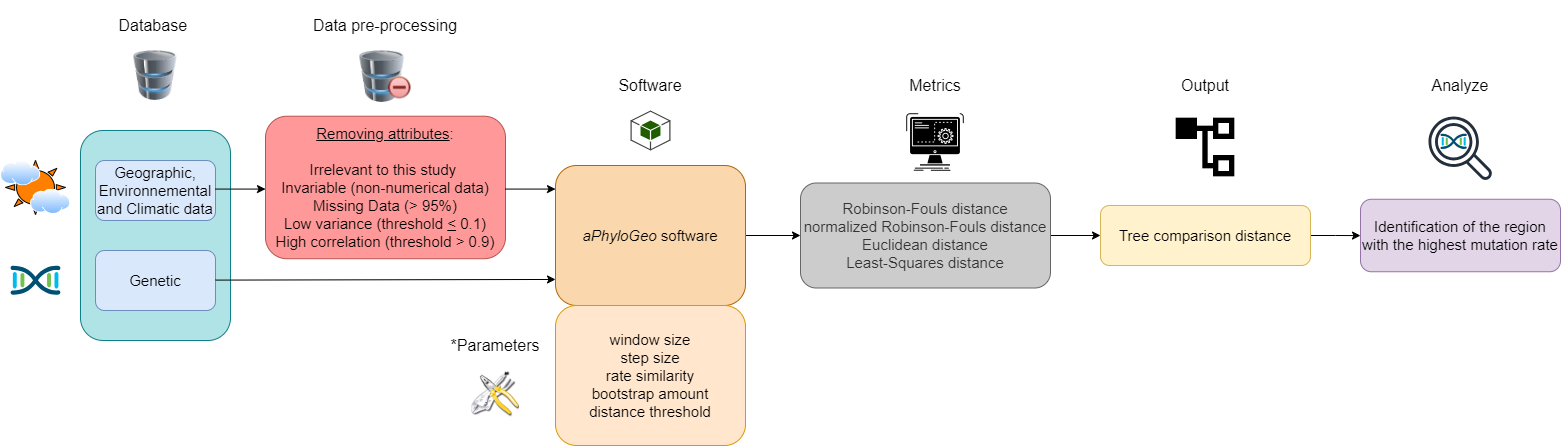
\includegraphics[width=0.7\textwidth]{diagram.drawio.png}
    \caption{Flow chart summarizing the Materials and Methods section workflow. Six different colors highlight the blocks. The first block (blue) represents our database. The second block (red) is data pre-processing, where we remove attributes. The third and fourth blocks (orange) implement the \textit{aPhyloGeo} software and its parameters for our phylogeographic analyses. The fifth block (grey) calculates phylogenetic tree comparison distances. The sixth block (yellow) compares the distances between the phylogenetic trees produced. The seventh block (purple) identifies regions with high mutation rates based on the results of the tree comparisons. *See YAML file on \href{https://github.com/tahiri-lab/aPhyloGeo}{GitHub}. \label{fig:fig1}}
\end{figure}

\subsection{Description of the data}

The study area was located in a northern region of the North Atlantic, including the Icelandic Sea, the Denmark Strait, and the Norwegian Sea. The specimens examined were collected as part of the IceAGE project (Icelandic marine Animals: Genetic and Ecology; Cruise ship M85/3 in 2011), which studied the deep continental slopes and abyssal waters around Iceland \citep{meisner_prefacebiodiversity_2018}. The sampling period for the included specimens was from August 30 to September 22, 2011, and they were collected at depths ranging from 316 to 2568 m. Information on the sampling plan, sample processing, DNA extraction steps, PCR amplification, sequencing, and extracted and aligned DNA sequences is available in the \citep{uhlir_adding_2021} article.

\subsection{Data pre-processing}

We used data from the IceAGE project and related data from the BOLD Systems database, both accessible \emph{via} the \citep{uhlir_adding_2021}. Given these databases' enormous breadth of attributes, we selectively reduced the number of attributes and samples. Specifically, we omitted attributes that were irrelevant in the context of this study, were entirely or nearly invariant (non-numerical data), and had a large number of missing data (>95\%). In the IceAGE dataset, we considered 62 specimens out of the 495 available. Next, we calculated the variance for each of the selected numerical attributes to eliminate those with zero or low variance (threshold ≤ 0.1). The equation \ref{variance} provides the variance formula used in this study.

\begin{equation}\label{variance}
    S^2 = \frac{\sum_{i=1}^{n} (x_i - \bar{x})^2}{n-1}
\end{equation}

where $S^2$ is the sample variance, $x_i$ represents each value in the dataset, $\bar{x}$ the mean of all values in the dataset, and $n$ the number of values in the dataset.

Only salinity was removed from the previously selected numerical attributes ($S^2 = 0.02146629$). We then removed attributes that had high correlations between them (threshold > 0.90). This selection of attributes and data resulted in a table containing 62 rows ($n=62$) and 20 columns (number of attributes). 

In the IceAGE database, 14 attributes were selected. These are the geographic coordinates such as: 

\begin{itemize}
\item The latitude and longitude taken at the start (see Figure \ref{fig:fig2}a and Figure \ref{fig:fig2}b) and end of sampling, both in decimal degrees (DD).
\item The geographical data are divided into five sectors across the seas around Iceland: the Denmark Strait ($n=28$), the Iceland Basin ($n=15$), the Irminger Basin ($n=12$), the Norwegian Sea ($n=4$), and the Norwegian Basin ($n=3$). 
\end{itemize}

For environmental features, we have included:
\begin{itemize}
\item Depth (m) at the start (see Figure \ref{fig:fig2}c) and end of sampling, as well as temperature ($^\circ$C) (see Figure \ref{fig:fig2}e) and O\textsubscript{2} concentration (mg/L) (see Figure \ref{fig:fig2}f) of the water as a function of the depth at which specimens were sampled. 
\item The sedimentary characteristics of the sampling sites, which influence the distribution of Cumacea \citep{uhlir_adding_2021}. In this study, they fall into six categories: mud ($n=30$), sandy mud ($n=15$), sand ($n=9$), forams ($n=3$), muddy sand ($n=3$), and gravel ($n=2$).
\end{itemize}

Climatic parameters such as: 
\begin{itemize}
\item Wind speed (m/s) (see Figure \ref{fig:fig2}d) and wind direction at the start and end of sampling were also included, given the contribution of wind to the restructuring of the benthic ecosystem through water transport \citep{waga_recent_2020,saeedi_environmental_2022}. The wind direction at the start of sampling comprises six orientations: South-West ($n=22$), South ($n=15$), North-East ($n=9$), South-South-East ($n=9$), North-West ($n=5$), and East ($n=2$); while that at the end of sampling is composed of seven orientations: South ($n=15$), South-West ($n=15$), North-East ($n=9$), West-South-West ($n=7$), South-East ($n=6$), North-North-West ($n=5$), South-South-East ($n=3$), and East ($n=2$). 
\end{itemize}

In the BOLD Systems database, taxonomic ranks such as: 
\begin{itemize}
\item The family, genus, and scientific name of the cumacean sampled have been integrated into our data. These comprise seven families: Diastylidae ($n=21$), Lampropidae ($n=13$), Leuconidae ($n=12$), Astacidae ($n=7$), Bodotriidae ($n=4$), Ceratocumatidae ($n=3$), and Pseudocumatidae ($n=2$). A total of 21 cumacean species were found in our sample (see Figure \ref{fig:fig3}).
\end{itemize}

We also included the sample identity (id) of each cumacean sampled. Some specimens were identified only to genus (one specimen) or family (five specimens) in our sample.
 
The habitat and water mass of the sampling points were the only attributes taken directly from Table 1 of \citep{uhlir_adding_2021}. Thus, the water mass definitions described by \citep{hansen_north_2000, brix2010distribution, ostmann_marine_2014} were used as a reference for the GIN seas around Iceland: Arctic Polar Water (APW, $n=15$), Iceland Sea Overflow Water (ISOW, $n=15$), North Atlantic Water (NAW, $n=9$), Arctic Polar Water/Norwegian Sea Arctic Intermediate Water (APW/NSAIW, $n=7$), warm Norwegian Sea Deep Water (NSDWw, $n=8$), Labrador Sea Water (LSW, $n=3$), cold Norwegian Sea Deep Water (NSDWc, $n=3$), and Norwegian Sea Arctic Intermediate Water (NSAIW, $n=2$) (see Figure \ref{fig:fig4}). In terms of habitat, we considered the three categories used in \citep{uhlir_adding_2021}: deep sea ($n=38$), shelf ($n=15$), and slope ($n=9$) (see Figure \ref{fig:fig5}).

To better interpret benthic species' relationship and evolutionary responses, genetic data are required \citep{wilson_speciation_1987, uhlir_adding_2021}. Thus, the aligned DNA sequence of the 16S rRNA mitochondrial gene region from each of the samples was included in our analyses. This region is standard in phylogeny and phylogeography studies \citep{hugenholtz1998impact} and sufficiently conserved over time to guarantee exact alignments between different species or populations \citep{saccone1999evolutionary}. We examined 62 of the 306 aligned DNA sequences used for phylogeographic analyses by \citep{uhlir_adding_2021}. As some specimens in our sample have their DNA sequence duplicated, or even quadruplicated with a difference of one or two nucleotides, we took into account the longest-aligned DNA sequence of each specimen.

Figure \ref{fig:fig2}, Figure \ref{fig:fig3}, Figure \ref{fig:fig6} and Figure \ref{fig:fig7} were made with Python 3.11, while Figure \ref{fig:fig4} and Figure \ref{fig:fig5} were made with RStudio Desktop 4.3.2.

\subsection{{\textit{aPhyloGeo} software}\label{aPhyloGeo-software}}

We used the cross-platform Python software \textit{aPhyloGeo} for our phylogeographic analyses, designed to analyze phylogenetic trees using ecological and geographic parameters. Developed by My-Linh Luu, Georges Marceau, David Beauchemin, and Nadia Tahiri, \textit{aPhyloGeo} offers tools to study correlations between species genetics and habitat characteristics, enabling us to understand the evolution of species under different environmental conditions. This software was chosen for our analysis because, to our knowledge, it is the first phylogeographic tool to correlate species genetics with climatic, environmental, and geographical attributes, which is the objective of our study. The \textit{aPhyloGeo} Python package is freely and publicly available on \href{https://github.com/tahiri-lab/aPhyloGeo}{GitHub}, and is also available on \href{https://pypi.org/project/aphylogeo/}{PyPi}, to facilitate complex phylogeographic analyses. The software process has three main stages (see \autoref{lst:main}).

%\autoref{lst:main}.
\begin{lstlisting}[label=lst:main,language=Python,caption=Main script for tutorial using the aPhyloGeo package.]
if __name__ == "__main__":

    # Load parameters
    Params.load_from_file()
    # Load the sequence file
    sequenceFile = utils.loadSequenceFile(Params.reference_gene_filepath)
    # Create an AlignSequences object
    align_sequence = AlignSequences(sequenceFile)

    # Load climatic data 
    climatic_data = pd.read_csv(Params.file_name)

    # Perform the alignment of sequences
    alignments = align_sequence.align()

    # Generate phylogenetic trees
    geneticTrees = utils.geneticPipeline(alignments.msa)
    
    # Create a GeneticTrees object
    trees = GeneticTrees(trees_dict=geneticTrees, 
                        format="newick")
   
    # Generate climatic trees (combines environmental, geographical, and climatic data)
    climaticTrees = utils.climaticPipeline(climatic_data)
    
    # Filter the results
    utils.filterResults(climaticTrees, 
                        geneticTrees, 
                        climatic_data)

\end{lstlisting}

\begin{enumerate}
\item \textbf{The first step} is to collect cumacean DNA sequences of sufficient quality for the needs of our results \citep{koshkarov_phylogeography_2022}. 62 cumaceans samples were selected to represent 62 16S rRNA mitochondrial gene sequences. We then included two climatic factors, namely wind speed (m/s) at the start and end of the sampling. We also included four environmental factors, such as sampling depth (m) at the start and end of sampling, temperature ($^\circ$C), and water O\textsubscript{2} concentration (mg/L). Finally, we integrated four geographical parameters, including latitude (DD) and longitude (DD) at the start and end of sampling.

\item \textbf{In the second step}, trees were generated with environmental, geographical, climatic, and genetic data. Concerning geographical parameters, we calculated the dissimilarity between each data pair from different geographical conditions, producing a symmetrical square matrix. The {neighbor-joining algorithm}\footnote{It is a method used to construct phylogenetic trees using distance matrices.} was used to design the geographic tree from this matrix. The same approach was applied to environmental, climatic, and genetic data. An {iterative phylogenetic reconstruction method}\footnote{This method makes it possible to build phylogenetic trees by progressively reforming them as new data or sequences are added.} was used to construct phylogenetic trees based on 62 16S rRNA mitochondrial sequences, taking into account only data located within an interval that moves along the alignment. This displacement can vary according to the steps and the size of the window defined by the user (their length is determined by the number of base pairs (bp)) \citep{koshkarov_phylogeography_2022}.

\item \textbf{In the third step}, the phylogenetic trees constructed in each sliding window are compared with environmental, climatic and geographical parameters using Robinson-Foulds distance (RF) \citep{robinson_comparison_1981, koshkarov_phylogeography_2022}, normalized Robinson-Foulds distance (nRF), Euclidean distance and Least-Squares distance (LS). These contribute to the understanding of similarities and dissimilarities between cumacean genetic sequences. The approach also takes bootstrapping into account. A sliding window allows detailed identification of regions with high genetic mutation rates.
\end{enumerate}

\section{Metrics}\label{metrics}

The following section presents a more concise version of the formulas mentioned in the third step of the \autoref{aPhyloGeo-software} section:

\subsection{Robinson-Foulds distance}\label{RF}

The Robinson-Foulds distance measures the dissimilarity between phylogenetic trees by counting the number of clades present in one tree but absent in the other. It is commonly used to quantify topological differences between phylogenetic trees (see Equation \eqref{eq:rf} and \autoref{lst:robinsonFoulds}).

When a gene tree is compared with other gene trees, all built using different habitat parameters (see the list in the first step of \autoref{aPhyloGeo-software}), the Robinson-Foulds distance can tell us how many clades differ between the initial tree and the others. When the initial phylogenetic tree constructed using one of the attributes shows strong dissimilarity with the other trees, this suggests that this parameter exerts an influence distinct from the others on the phylogenetic relationships of cumacean species.

\begin{equation}\label{eq:rf}
    \text{RF}(T_1, T_2) = | \Sigma(T_1) \Delta \Sigma(T_2) |
\end{equation}

where $\Sigma(T_1)$ and $\Sigma(T_2)$ are the sets of splits in trees $T_1$ and $T_2$.

%\autoref{lst:robinsonFoulds}.
\begin{lstlisting}[label=lst:robinsonFoulds,language=Python,caption=Python script for calculating the Robinson-Foulds distance using the ete3 package in the aPhyloGeo package.]
    def robinsonFoulds(tree1, tree2):
        rf = 0
        tree1_newick = ete3.Tree(tree1.format("newick"), format=1)
        tree2_newick = ete3.Tree(tree2.format("newick"), format=1)

        rf, rf_max, common_leaves = tree1_newick.robinson_foulds(tree2_newick, 
                                                                 unrooted_trees=True)
        if len(common_leaves) == 0:
            rf = 0

        return rf, rf / rf_max
\end{lstlisting}


\subsection{Normalized Robinson-Foulds distance}\label{RFnorm}

The normalized Robinson-Foulds distance scales the RF distance to account for the size  of the trees (number of clades), allowing a fairer comparison and giving a value between 0 and 1. In this case, the distance has been normalized by $2n-6$, where $n$ represents the number of taxa, to make it easier to compare the relative differences between trees (see Equation \eqref{eq:rf_norm} and \autoref{lst:euclideanDist}).

If the phylogenetic trees are of different sizes (e.g., if one of them is based on a missing data set or a reduced number of species or parameters), the nRF distance makes it possible to interpret the relative influence of each habitat feature on the evolutionary relationships of cumacean, independently of the number of clades in the trees.

\begin{equation}\label{eq:rf_norm}
    \text{RF}_{\text{norm}}(T_1, T_2) = \frac{| \Sigma(T_1) \Delta \Sigma(T_2) |}{| \Sigma(T_1) | + | \Sigma(T_2) |}
\end{equation}

\subsection{Euclidean distance}\label{euclidean}

Euclidean distance measures the length between two points in a multi-dimensional space. In our study, it is used to parallel the vectors of habitat characteristics between species (see Equation \eqref{eq:euclidean} and \autoref{lst:euclideanDist}).

When the values of different habitat features are converted into vectors, Euclidean distance allows us to understand how combinations of various habitat attributes integrally affect the phylogenetic trees of cumacean species. For example, species with similar environmental or climatic vectors (low Euclidean distance) may have close evolutionary relationships. On the other hand, large dissimilarities in these vectors (high Euclidean distance) can signify significant evolutionary differences.

For points $\mathbf{p} = (p_1, \ldots, p_n)$ and $\mathbf{q} = (q_1, \ldots, q_n)$:

\begin{equation}\label{eq:euclidean}
    d_{\text{Euclidean}}(\mathbf{p}, \mathbf{q}) = \sqrt{\sum_{i=1}^{n} (p_i - q_i)^2}
\end{equation}

%\autoref{lst:euclideanDist}.
\begin{lstlisting}[label=lst:euclideanDist,language=Python,caption=Python script for calculating the Euclidean distance using the ete3 package in the aPhyloGeo package]
    def euclideanDist(tree1, tree2):
        
        tns = dendropy.TaxonNamespace()
        
        tree1_tc = dendropy.Tree.get(data=tree1.format("newick"), 
                                     schema="newick", 
                                     taxon_namespace=tns)
                                     
        tree2_tc = dendropy.Tree.get(data=tree2.format("newick"), 
                                     schema="newick", 
                                     taxon_namespace=tns)
                                     
        tree1_tc.encode_bipartitions()
        tree2_tc.encode_bipartitions()

        ed = dendropy.calculate.treecompare.euclidean_distance(tree1_tc, tree2_tc)

        return ed
\end{lstlisting}

\subsection{Least-Squares distance}\label{LS}

The Least squares distance measures differences by considering the sum of the squares of the differences between the observed values and the estimated values provided by the model. In our context, when comparing a phylogenetic tree with other trees, all constructed using different habitat factors, it quantifies the overall topological dissimilarity of the initial phylogenetic tree, taking into account the position of nodes and branches (see Equation \eqref{eq:ls} and \autoref{lst:LeastSquare}).

Least-squares distance allows us to elucidate the specific influences of various attributes on tree composition concerning branch position and length, and to reform evolutionary links between cumacean species.

For observed values $y_i$ and estimated values $\hat{y}_i$:

\begin{equation}\label{eq:ls}
    d_{\text{LS}} = \sum_{i=1}^{n} (y_i - \hat{y}_i)^2
\end{equation}

%\autoref{lst:LeastSquare}.
\begin{lstlisting}[label=lst:LeastSquare, language=Python, caption=Python script for calculating the Least-Square distance using the ete3 package in the aPhyloGeo package]
def least_square(tree1, tree2):
    ls = 0.0
    leaves = tree1.get_terminals()

    leaves_name = list(map(lambda x: x.name, leaves))
    for i in leaves_name:
        leaves_name.pop(0)
        for j in leaves_name:
            d1 = tree1.distance(tree1.find_any(i), tree1.find_any(j))
            d2 = tree2.distance(tree2.find_any(i), tree2.find_any(j))
            ls += abs(d1 - d2)
    return ls
\end{lstlisting}

Our phylogeographic study used these four metrics to quantify topological differences between phylogenetic trees and assess dissimilarities between genetic sequences and environmental, geographical, and climatic features. The result is a comprehensive analysis of the evolutionary dynamics of cumacean populations in different contexts.

\section{Results}\label{results}

To understand the correlation between cumacean genetics and habitat, we parameterized the software \textit{aPhyloGeo} as follows: pairwiseAligner, Hamming distance, Wider Fit by elongating with Gap (starAlignment), windows size: 1 nucleotide (nt) and window step: 10 nt. The results of the metrics used were obtained using the functions leastSquare(tree1, tree2), robinsonFoulds(tree1, tree2), euclideanDist(tree1, tree2) from the \textit{aPhyloGeo} software and were organized by the main function (see \autoref{lst:main}). A more in-depth analysis of the results presented below is available on \href{https://github.com/tahiri-lab/Cumacea_aPhyloGeo}{GitHub} in the supplementary file.

The violon diagrams shown in Figure \ref{fig:fig2} are used to display summary statistics similar to box plots, showing medians (white dots), interquartile ranges (thickened black bars), and the rest of the distributions (thin black lines), except the "extreme" points. Wider areas indicate a greater probability of the variables taking a given value. They illustrate the distribution of geographical (latitude and longitude at the start of sampling (DD)), climatic (wind speed (m/s) at the start of sampling), and environmental (depth (m) at the start of sampling, water temperature ($^\circ$C), and O\textsubscript{2} concentration (mg/L)) data. These diagrams are essential for understanding habitat conditions and highlighting unique habitats that may impact cumacean genetics. 

\begin{figure}[htbp]
    \centering
    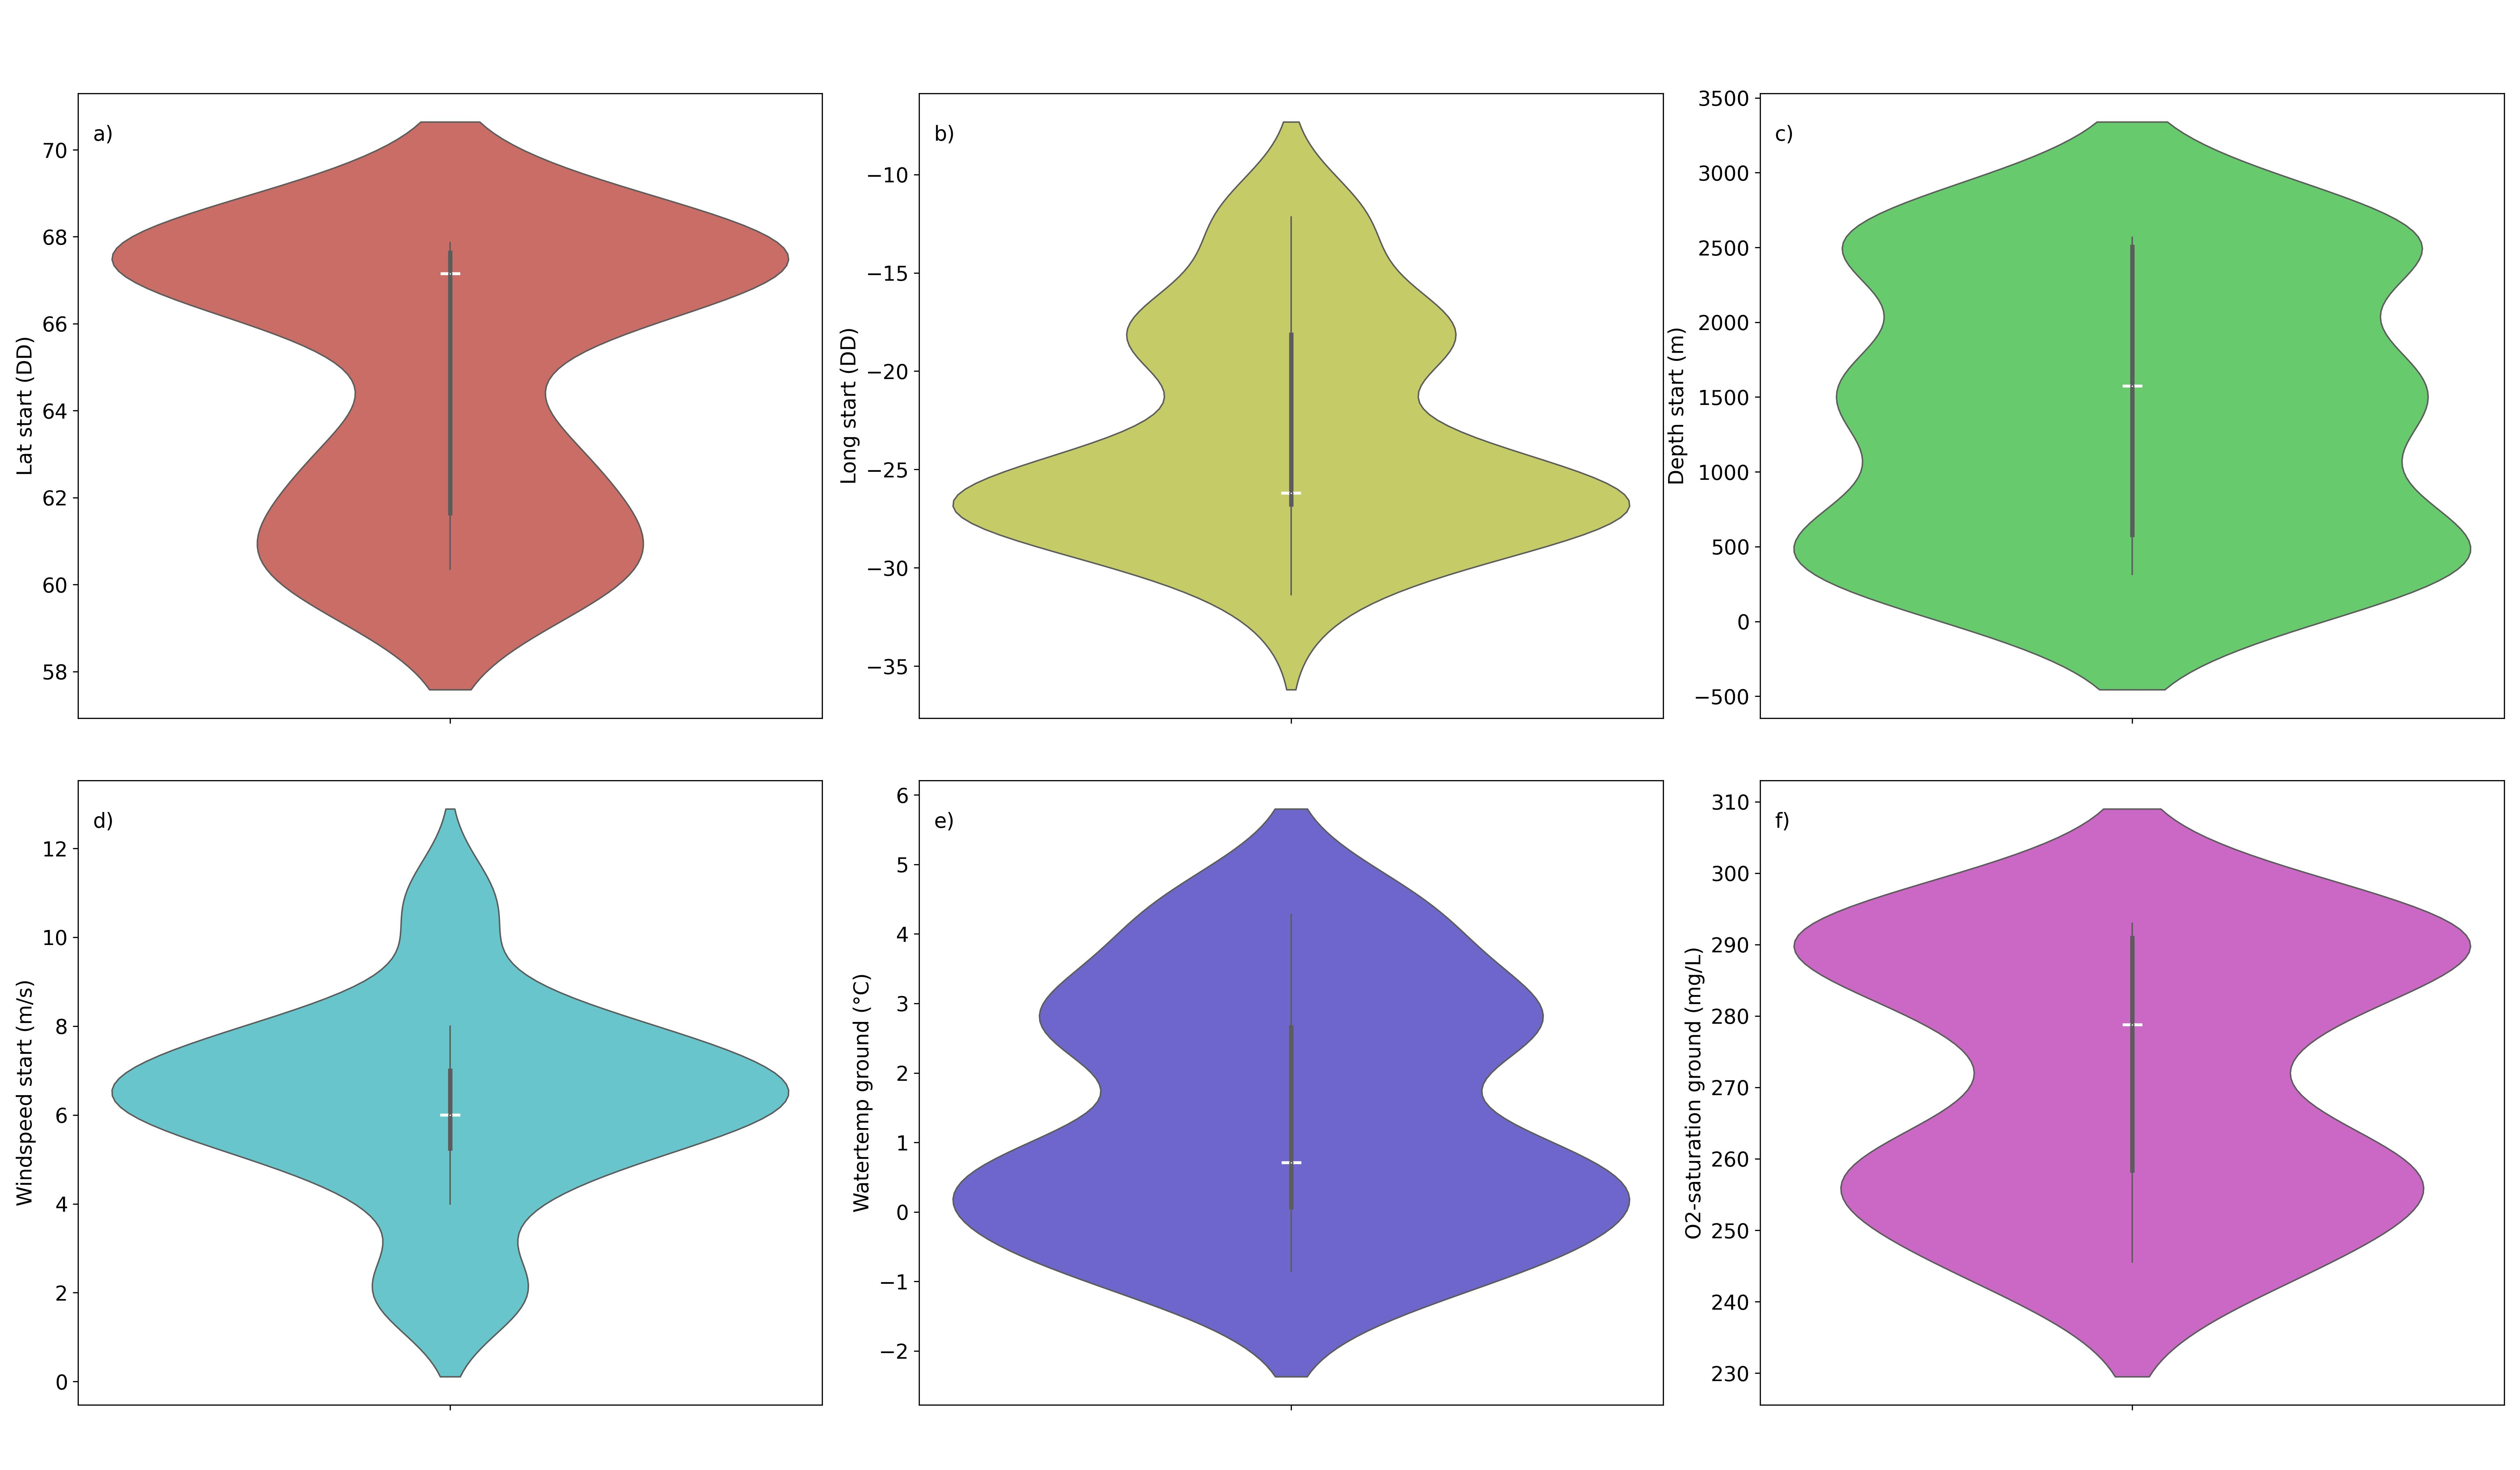
\includegraphics[width=0.7\textwidth]{figure1.jpg}
    \caption{Violin diagrams of two geographical attributes, one climatic attribute, and three environmental attributes from our sample. a) Latitude (DD) at the start of sampling (red); b) Longitude (DD) at the start of sampling (yellow); c) Depth (m) at the start of sampling (green); d) Wind speed (m/s) at start of sampling (light blue); e) Water temperature ($^\circ$C) as a function of depth at which specimens were collected (dark blue); f) O\textsubscript{2} concentration (mg/L) as a function of depth at which specimens were sampled (pink). The mean, median, standard deviation (Std Dev), 1st quartile (Q1), and 3rd quartile (Q3) of the dataset for each attribute are shown in the top right-hand corner of each graph. \label{fig:fig2}}
\end{figure}

Our results revealed environmental variability in most cumacean habitat attributes in Figure \ref{fig:fig2}. The median of Figure \ref{fig:fig2}a (67.15 DD) is higher than the mean (64.83 DD), indicating an asymmetric distribution towards lower values. This is also the depth case (m) at the start of sampling and water (O\textsubscript{2} concentration (mg/L) (see Figure \ref{fig:fig2}c and Figure \ref{fig:fig2}f). The curve in Figure \ref{fig:fig2}a has an asymmetrical bimodal shape, showing two peaks, suggesting that the samples came from two dominant latitudinal regions at the start of sampling. This could indicate important fluctuations in climatic and environmental conditions in the sampled areas. Similarly, this type of curve is present for longitude (DD) at the start of sampling, as well as for temperature ($^\circ$C) and O\textsubscript{2} concentration (mg/L) of the water from which the samples were taken (see Figure \ref{fig:fig2}b, Figure \ref{fig:fig2}e and Figure \ref{fig:fig2}f). 

The median in Figure \ref{fig:fig2}b (-26.21 DD) is lower than the mean (-23.12 DD), indicating asymmetry on the higher sides, as does the water temperature ($^\circ$C) (see Figure \ref{fig:fig2}e). The standard deviation (5.52 DD) and quartiles Q1 (-26.77 DD) and Q3 (-18.14 DD) indicate a relatively wide range, around the mean (-23.12 DD), of the longitude distribution at the start of sampling (-31.356 - -12.162 DD). This suggests a strong environmental gradient, geographical distribution and sample diversity from east to west in the region studied. The standard deviation of Figure \ref{fig:fig2}c is quite high (881.16 m), indicating high variability in sample collection depths (316 – 2568 m) and giving a more global overview of benthic habitats. Unlike all the other diagrams in Figure \ref{fig:fig2}, the curve in Figure \ref{fig:fig2}c has a multimodal shape with three prominent peaks, suggesting that the samples were mainly collected and concentrated at three different depths (around 500, 1500 and 2500 m).

The mean (6.26 m/s) and median (6.00 m/s) in Figure \ref{fig:fig2}d are the only ones in Figure \ref{fig:fig2} to be similar, indicating a symmetrical distribution, with a high concentration of data around the median (6.00 m/s). This suggests stable wind conditions (m/s) at the start of sampling. The standard deviation of Figure \ref{fig:fig2}e is relatively high (1.73 $^\circ$C) compared to the mean (1.45 $^\circ$C), indicating a wide range of water temperatures where samples were taken (0.851 – 4.28 $^\circ$C). This suggests the acclimatization of cumacean to a variety of habitat temperatures. The range of O\textsubscript{2} concentration data (see Figure \ref{fig:fig2}f) shows some variability (245.53 – 292.97 mg/L) in the environmental conditions of the sampled areas, as shown by the standard deviation (18.11 mg/L) and quartiles Q1 (258.39 mg/L) and Q3 (290.90 mg/L). These latest results reflect a diversity of O\textsubscript{2} requirements, with organisms adapted to low O\textsubscript{2} conditions and potentially influenced by the heterogeneity of biogeochemical cycles, such as photosynthesis, respiration, and organic decomposition, which have an impact on depth-dependent dissolved  O\textsubscript{2} levels.

\begin{figure}[htbp]
    \centering
    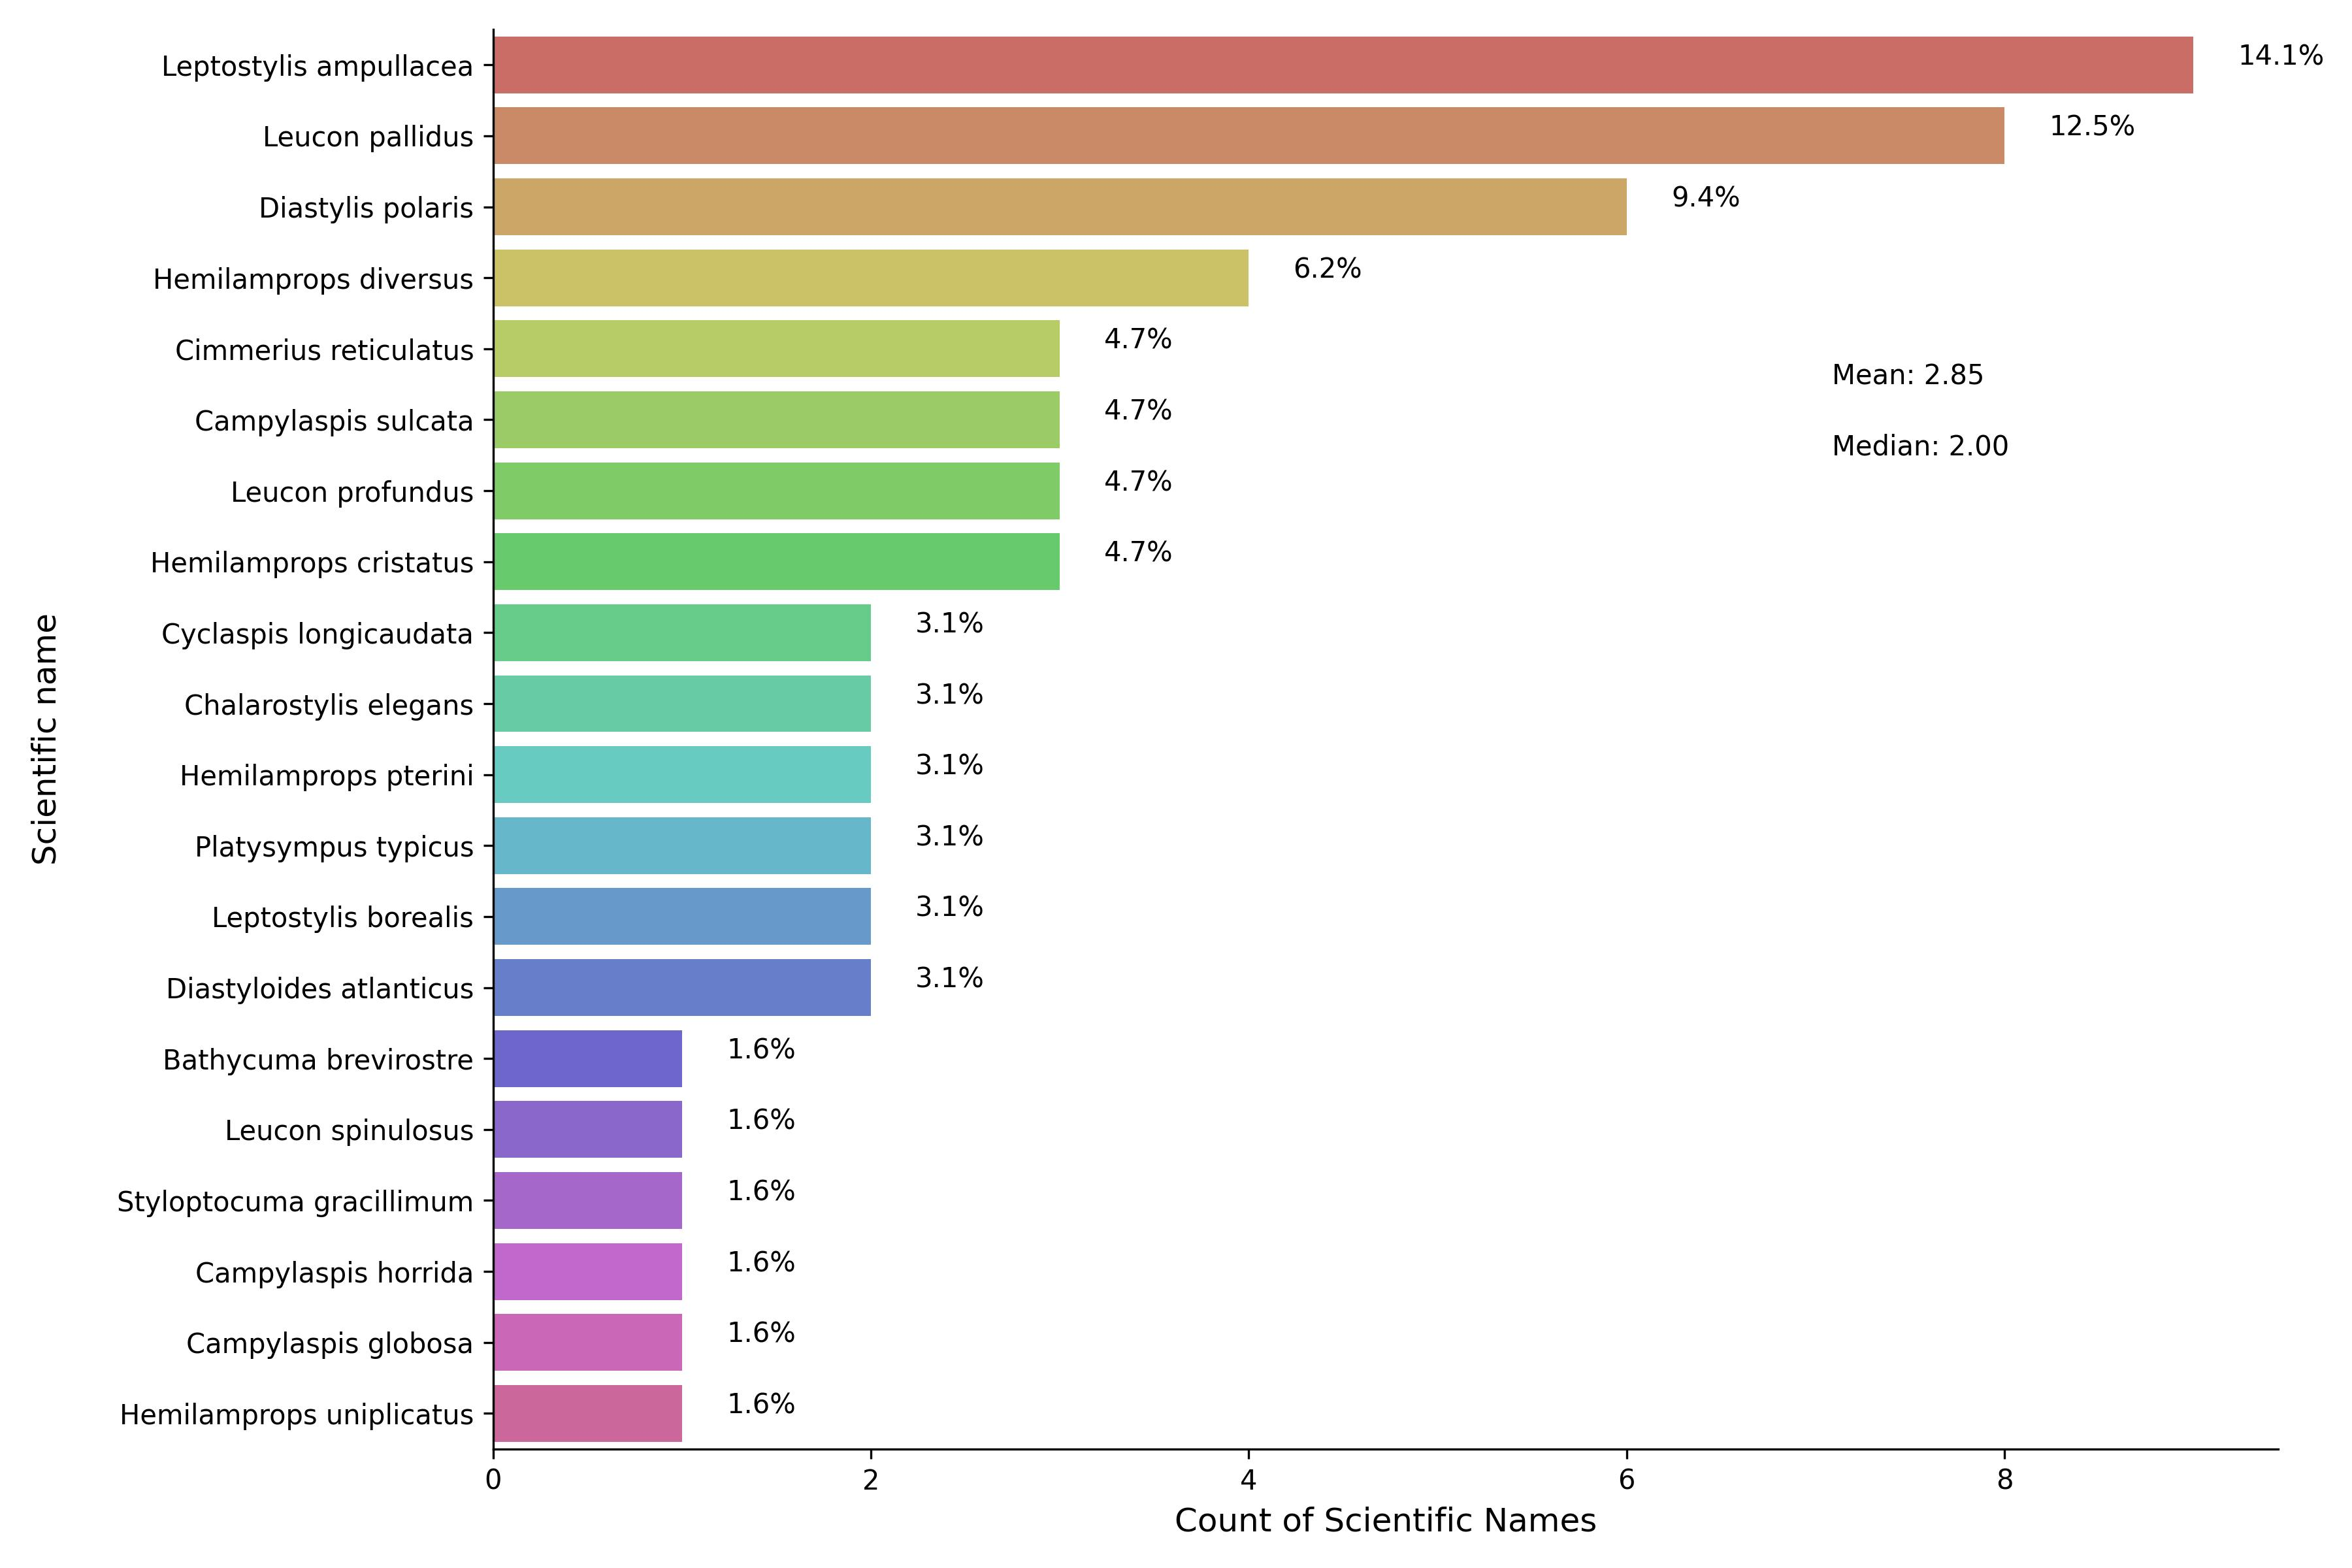
\includegraphics[width=0.7\textwidth]{figure2.jpg}
    \caption{Frequency distribution of cumacean species in our sample. The bars represent the number of individuals for each species. The percentages (\%) displayed above the bars indicate the relative abundance of each species in the total sample. The mean and median values of the frequency distribution are shown in the top right-hand corner of the histogram. \label{fig:fig3}}
\end{figure}

The distribution and diversity of the various cumacean species found in our sample are shown in Figure \ref{fig:fig3}. It shows the most represented species (\emph{Leptostylis ampullacea}, 14.1\%; \emph{Leucon pallidus}, 12.5\%) and the least represented species (\emph{Bathycuma brevirostre}, \emph{Leucon spinulosus}, \emph{Styloptocuma gracillimum}, \emph{Campylaspis horrida}, \emph{Campylaspis globosa}, and \emph{Hemilamprops uniplicatus}; all 1.6\%), suggesting particular ecological forces favoring or limiting certain species, or that some species have a restricted niche. Unlike less represented species, dominant species may have particular adaptive traits that favor their exploitation of food, interspecific competition, or resistance to changing environmental conditions.

\begin{figure}[htbp]
    \centering
    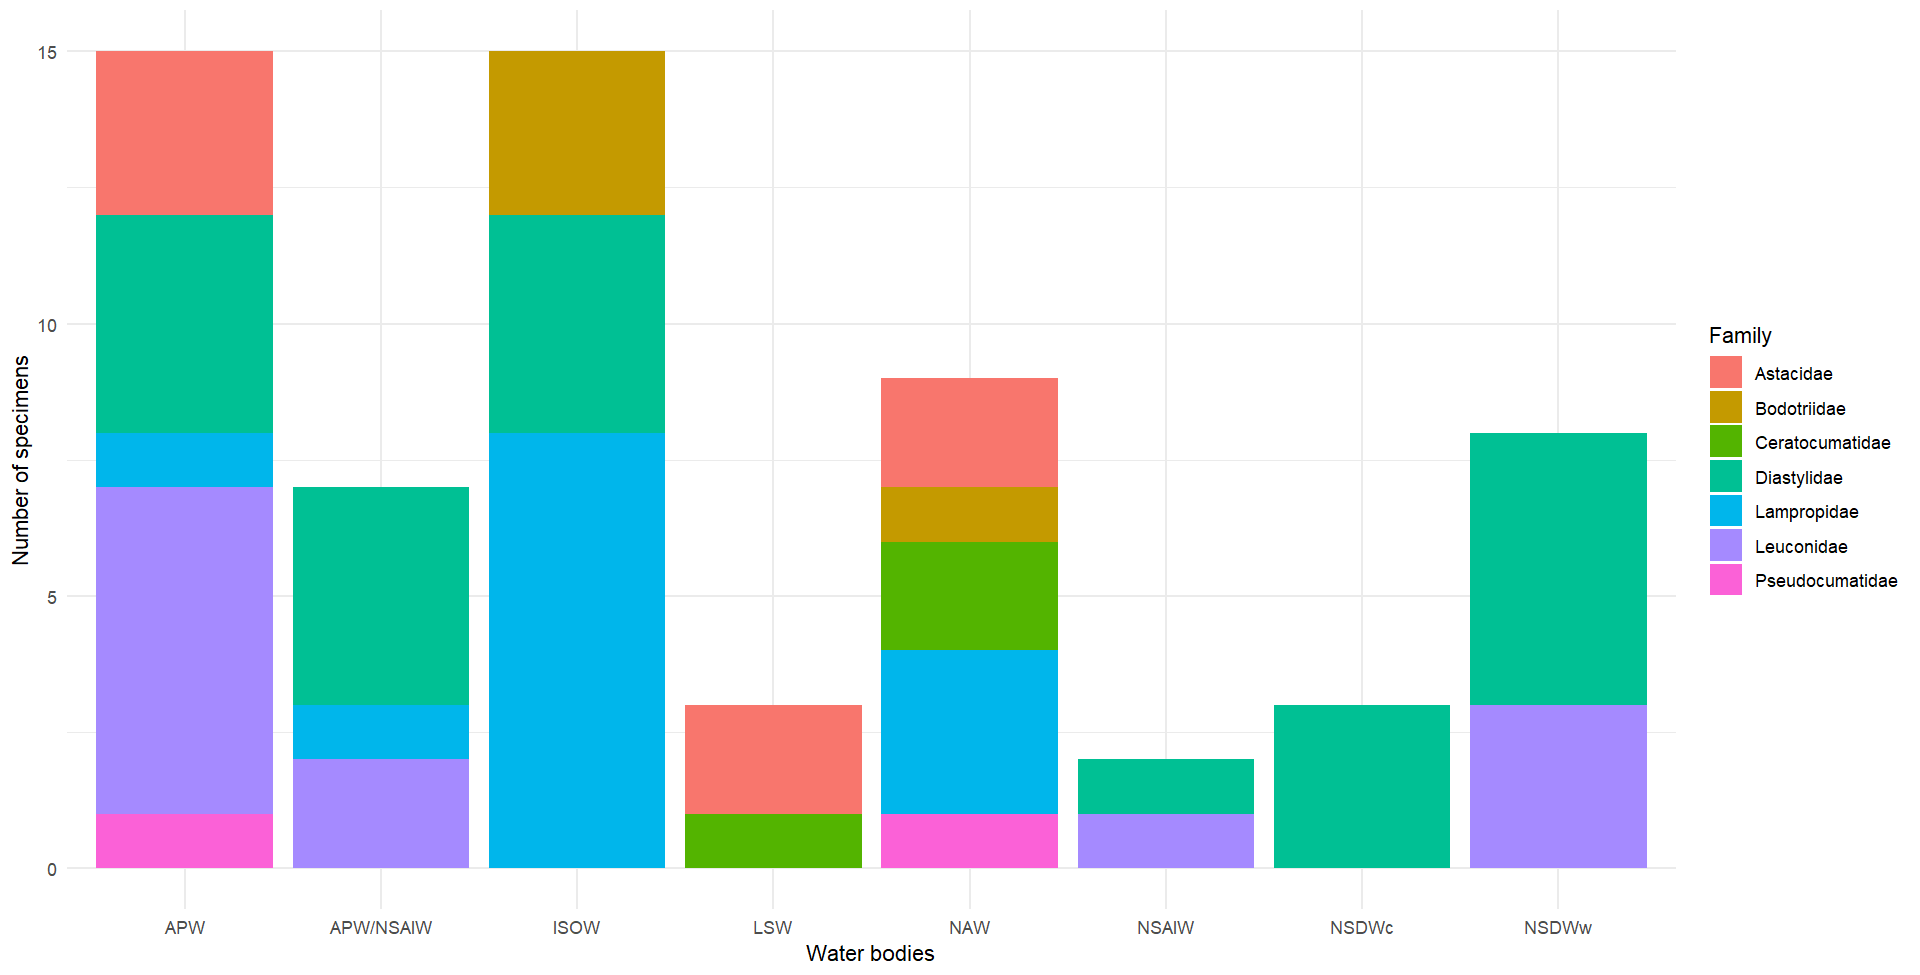
\includegraphics[width=0.7\textwidth]{figure3.png}
    \caption{Distribution of cumacean families by water mass. This histogram represents the frequency of occurrence of the different cumacean families in our samples, classified according to the water mass in which they were collected. Eight water mass categories are represented: Arctic Polar Water (APW), Arctic Polar Water/North Sub-Arctic Intermediate Water (APW/NSAIW), Iceland Scotland Overflow Water (ISOW), Labrador Sea Water (LSW), North Atlantic Water (NAW), North Sub-Arctic Intermediate Water (NSAIW), cold North Sub-Atlantic Deep Water (NSDWc), and warm North Sub-Atlantic Deep Water (NSDWw). Seven families are represented: Astacidae (red), Bodotriidae (brown), Ceratocumatidae (green), Diastylidae (turquoise), Lampropidae (blue), Leuconidae (purple), and Pseudocumatidae (pink). \label{fig:fig4}}
\end{figure}

The distribution of samples from the different cumacean families according to the variety of water masses in which they were collected is illustrated in Figure \ref{fig:fig4}. This allows us to compare the diversity and potential preferences of the different families in each water mass, with the Diastylidae family being the most present in all water masses (turquoise color). This testifies to the resilience and ecological adaptability of the Diastylidae family to a wide variety of environmental conditions, reminiscent of \emph{Leptostylis ampullacea} in Figure \ref{fig:fig3} which belongs to the Diastylidae family. Two water masses contain the greatest diversity of cumacean families, with Arctic Polar Water (APW) and North Atlantic Water (NAW) both with five families; APW: Astacidae, Diastylidae, Lampropidae, Leuconidae and Pseudocumatidae; NAW: Astacidae, Bodotriidae, Ceratocumatidae, Diastylidae, Lampropidae and Pseudocumatidae. This concomitance of different families could be explained by the diversified and resource-rich environments of these two water masses, favoring various complex ecological niches exploited by these families.

\begin{figure}[]
    \centering
    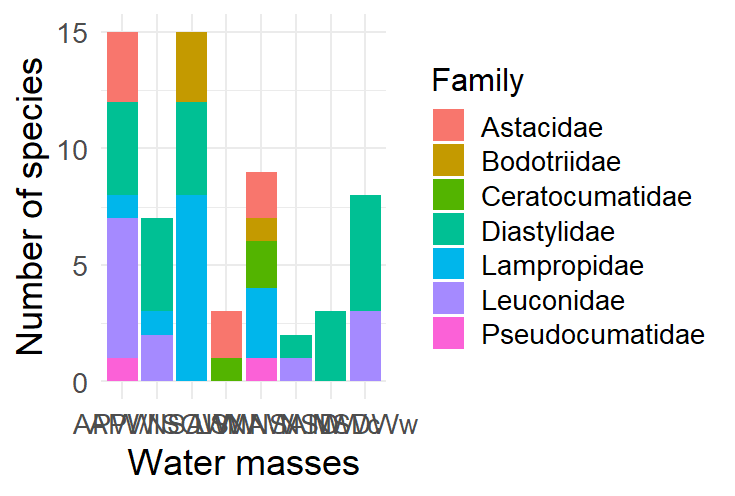
\includegraphics[width=0.7\textwidth]{figure4.png}
    \caption{Distribution of cumacean families by habitat. This histogram represents the frequency of occurrence of the different cumacean families in our samples, classified according to the habitat in which they were collected. Three habitat categories are represented: Deep sea, Shelf, and Slope. Seven families are represented: Astacidae (red), Bodotriidae (brown), Ceratocumatidae (green), Diastylidae (turquoise), Lampropidae (blue), Leuconidae (purple), and Pseudocumatidae (pink). \label{fig:fig5}}
\end{figure}

The distribution of samples of the different cumacean families according to the type of habitat where they were collected during sampling is shown in Figure \ref{fig:fig5}. Mainly dominated by Diastylidae and Lampropidae, a wide variety of families can be found in deep waters, which offer different ecological niches. The shelf also features some diversity of families, but less so than in the deep sea, with Leuconidae being the most abundant and acclimatized to these environmental conditions. The slope presents the lowest diversity of families, with a greater presence of Diastylidae, suggesting less varied ecological niches for cumaceans. The strong presence of families in particular habitats, such as the Diastylidae in the deep sea and on the slope, and the Leuconidae on the shelf, suggests that these families have acquired adaptive characteristics (physiological, behavioral, or morphological), which could favor their survival in these specific environments. It also recommends that accessible resources (food and ecological niches) and environmental conditions, such as temperature, O\textsubscript{2} concentration, and sediment type, are key factors in the distribution of cumacean families.

\begin{figure}[]
    \centering
    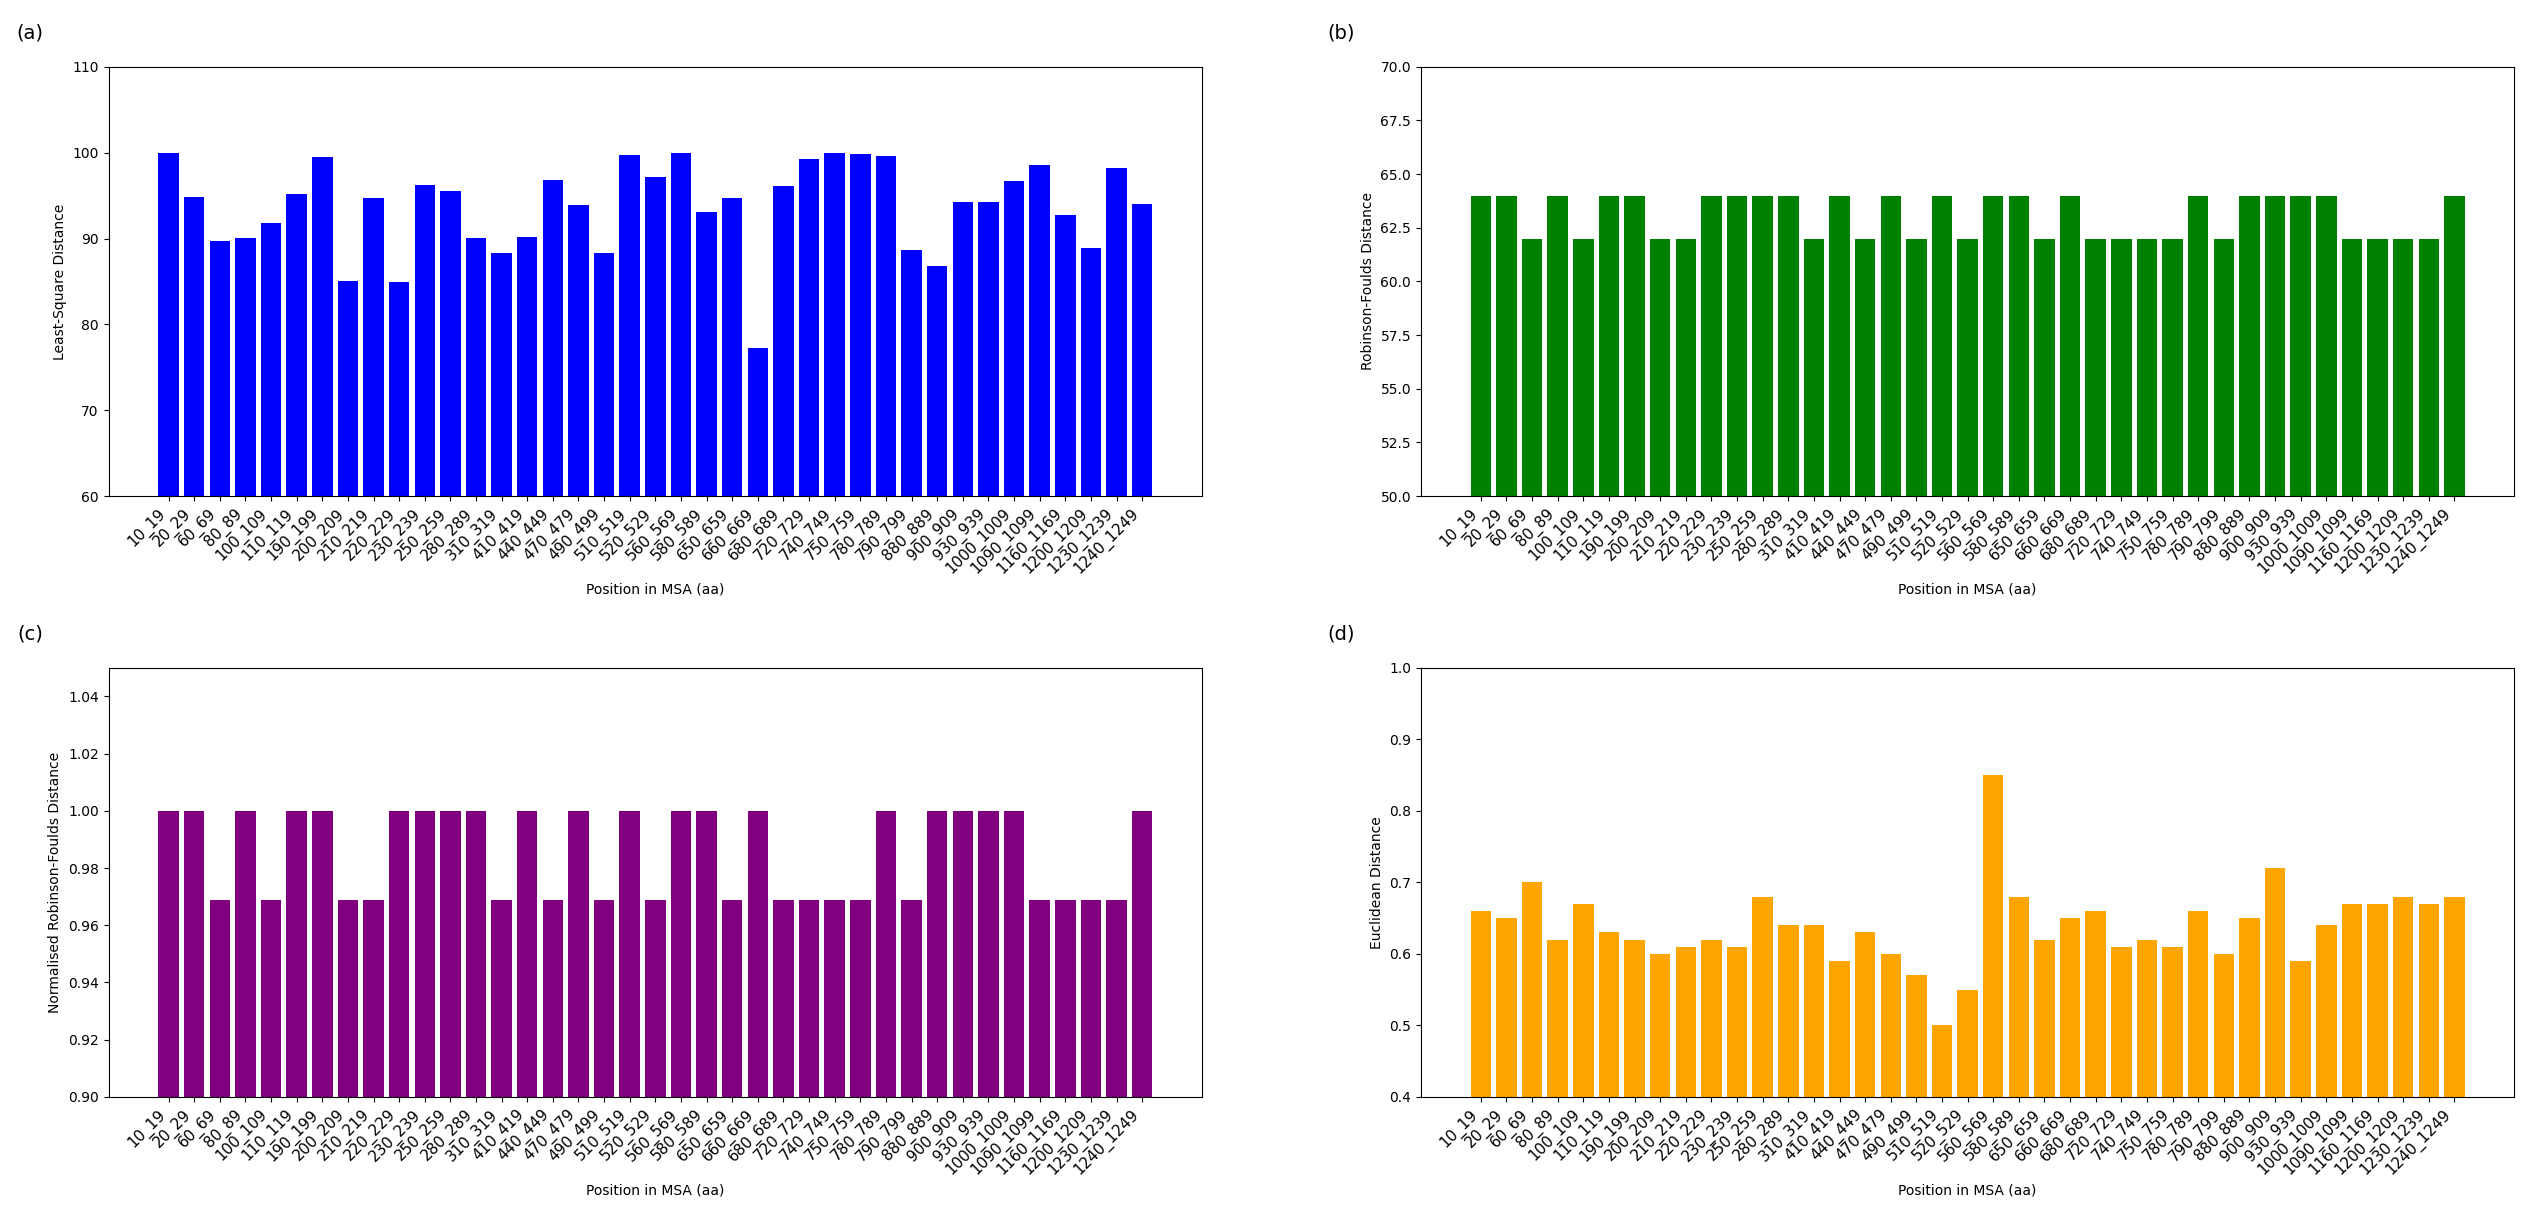
\includegraphics[width=0.7\textwidth]{figure5.png}
     \caption{Analysis of fluctuations in four distance metrics using multiple sequence alignment (MSA): a) Least-Squares (LS) distance, b) Robinson-Foulds (RF) distance, c) normalized Robinson-Foulds (nRF) distance, and d) Euclidean distance. These distance variations are studied to establish their correlation with the variation in wind speed (m/s) at the start of sampling. \label{fig:fig6}}
\end{figure}

\begin{figure}[]
    \centering
    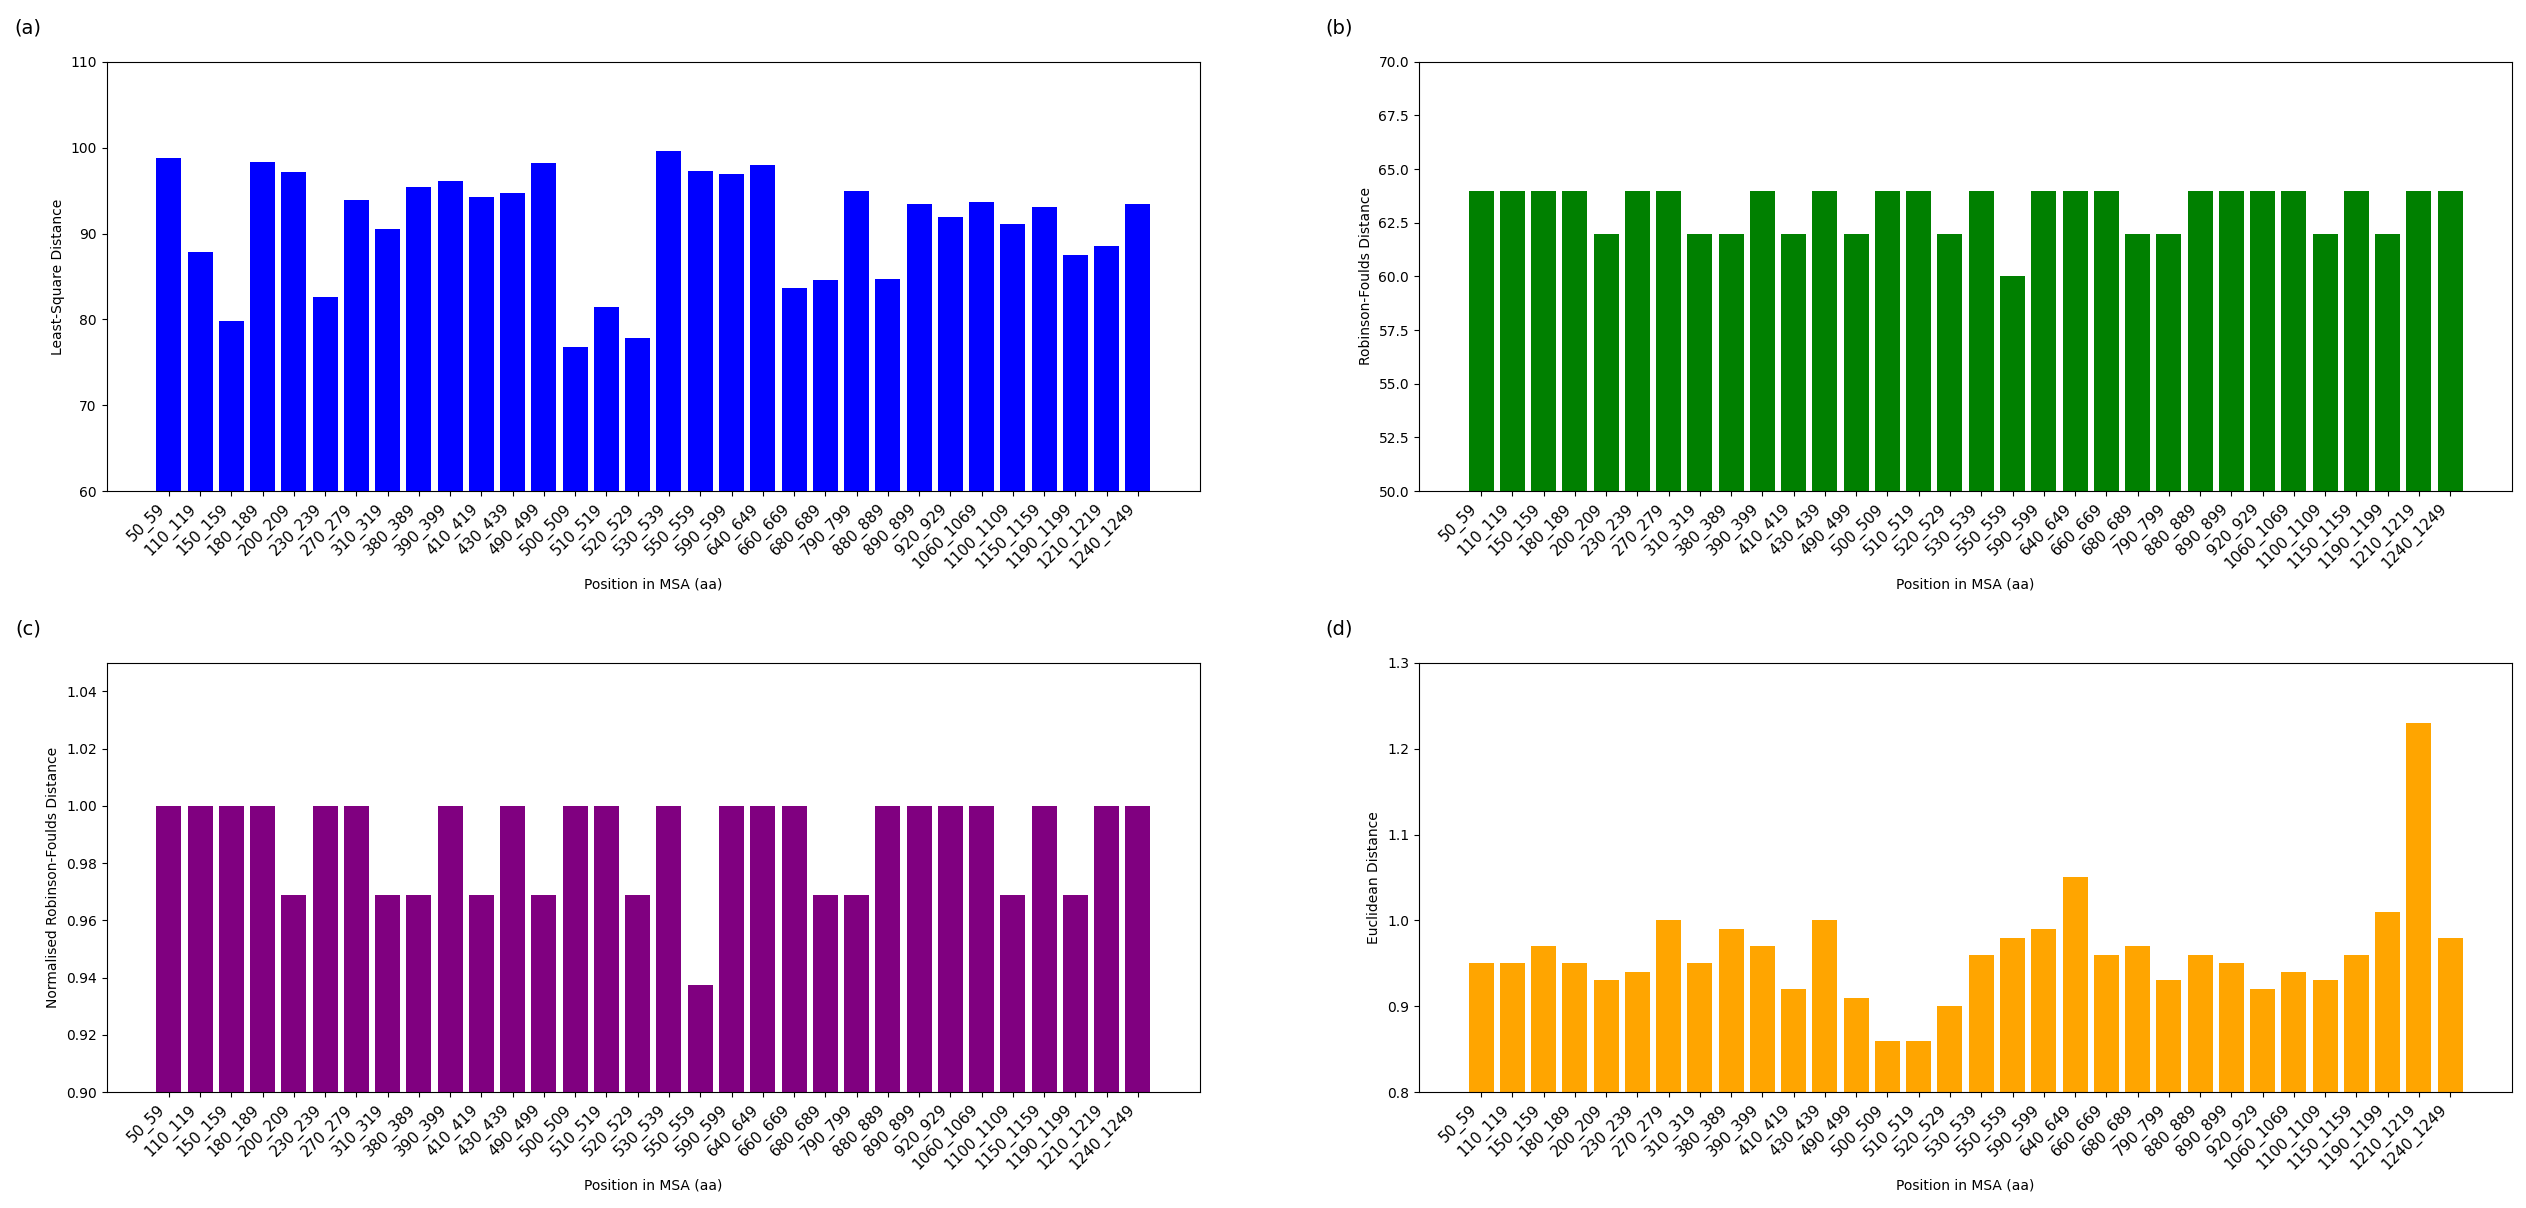
\includegraphics[width=0.7\textwidth]{figure6.png}
    \caption{Analysis of fluctuations in four distance metrics using multiple sequence alignment (MSA): a) Least-Squares (LS) distance, b) Robinson-Foulds (RF) distance, c) normalized Robinson-Foulds (nRF) distance, and d) Euclidean distance. These distance variations are studied to establish their correlation with variation of O\textsubscript{2} concentration (mg/L) at the sampling sites. \label{fig:fig7}}
\end{figure}

The correlation between the genetic sequences and two attributes, one climatic (wind speed (m/s) at the start of sampling) and the other environmental (O\textsubscript{2} concentration (mg/L)) is presented in Figure \ref{fig:fig6} and Figure \ref{fig:fig7}. These correlations are based on four distance metrics: LS, RF, nRF, and Euclidean. All the attributes presented in the first step of the \textit{aPhyloGeo} software section were analyzed (see \autoref{aPhyloGeo-software}) and are available on \href{https://github.com/tahiri-lab/Cumacea_aPhyloGeo}{GitHub} in the img and script python file. However, only these two parameters showed the most interesting mutation rate. Fluctuations in these parameters reflect an adaptive response of these specific genetic sequences to environmental and climatic conditions. In both Figures, Euclidean distance seems to be the most sensitive and heterogeneous according to our data. A higher Euclidean distance means a greater difference between sequences at positions 520 to 529 amino acids (aa) (see Figure \ref{fig:fig6}d) and 1190 to 1199 aa (see Figure \ref{fig:fig7}d), suggesting that these sites are more variable due to numerous mutations, subject to selection pressures or susceptible to evolutionary change. 

All these results will need to be studied and analyzed in greater depth to gain a better understanding and draw firm conclusions. In addition, we would like to know if they support the results of \citep{uhlir_adding_2021} on the influence of climatic and environmental factors on the distribution and genetics of Cumacea.

\section{Conclusion}\label{conclusion}

This study focuses on the effect of climatic, geographical, and environmental characteristics on the genetics of cumacean in the waters around Iceland. Our main objective is to establish whether there is a  correlation between the genetic information of the 16S rRNA mitochondrial gene region (i.e., window) of cumacean species and their habitat characteristics. We seek to identify the attribute most correlated with a specific genetic sequence and the potentially associated protein.

We laboriously selected relevant attributes from IceAGE project data, BOLD Systems, and the \citep{uhlir_adding_2021} article. We eliminated those that were not relevant to this study, as well as those with low variance (e.g., salinity, $S^2 = 0.02146629$), abundant missing data (> 95\%), and high correlation between them (threshold > 0.9). Using this refined dataset, we have integrated phylogeographic studies using \textit{aPhyloGeo} software (see \autoref{lst:main}), allowing us to analyze potential correlations between species genetics and environmental contexts.

Our results revealed variability in the cumacean environment according to attributes including longitude (DD) at the start of sampling, depth (m) at the beginning of sampling, temperature ($^\circ$C), and water O\textsubscript{2} concentration (see Figure \ref{fig:fig2}b, Figure \ref{fig:fig2}c, Figure \ref{fig:fig2}e and Figure \ref{fig:fig2}f). Particularly, DNA sequence analyses revealed specific genetic windows with elevated mutation rates in response to climatic and environmental attributes, such as wind speed (m/s) at the start of sampling and O\textsubscript{2} concentration in water (mg/L) (see Figure \ref{fig:fig6}d and Figure \ref{fig:fig7}d), indicating sensitive or variable sites in their evolutionary development.

The novelty of our study lies in the exhaustive correlation between ecological and geographic attributes and genetic mutability, especially  
Correlations can be used to explain how these organisms acclimatize to the documentation of genetic windows related to environmental change. This represents a considerable advance over previous studies, which have not examined these specific relationships in depth. The implications of our results are essential for interpreting how cumacean species adapt to climate change and anthropogenic disturbance, providing a potential basis for conservation plans. For instance, the management of fishing and mining activities could use these insights to diminish their impact on benthic species.

In addition, our research provides fundamental knowledge that can guide future studies on the genetic adaptation of cumaceans and other invertebrates to environmental variability. By emphasizing the importance of incorporating more environmental and climatic attributes, such as nutrient accessibility, water pH, ocean currents, and human disturbance, we establish a wider exploration that could further explain genotype-environment interactions

However, while further analysis of these results is required for this study, it is necessary to mention the limitations, notably the three missing data on O\textsubscript{2} concentration (mg/L) in water and the relatively small sample size ($n=62$). These factors could have an impact on our results and interpretations. Future studies should aim to fill these gaps, broadening the scope to other invertebrate species and geographical regions, to better understand the gene-environment interactions and their implications for marine biodiversity preservation.

\section{Acknowledgments}\label{acknowledgments}

The authors thank the SciPy conference and reviewers for their valuable comments on this paper as well as Mansour Kebe for his technical support and Carolin Uhlir for her clarifications and advice on her study \citep{uhlir_adding_2021}. This work was supported by the Natural Sciences and Engineering Research Council of Canada (NSERC), the Fonds de recherche du Québec - Nature et technologies (FRQNT), the Université de Sherbrooke grant, and the Centre de recherche en écologie de l’Université de Sherbrooke (CREUS).
